\chapter[A$\beta$42]{Molecular Mechanism of A$\beta$42 fibril inhibition by inositol}

% Some notes
% I found these pretty neat ref articles on sciencedirect
% http://www.sciencedirect.com.myaccess.library.utoronto.ca/science/article/pii/B9780444519672001550
% http://www.sciencedirect.com.myaccess.library.utoronto.ca/science/article/pii/B9780444519672000581
% http://www.sciencedirect.com.myaccess.library.utoronto.ca/science/article/pii/B9780444519672000313
% http://www.sciencedirect.com.myaccess.library.utoronto.ca/science/article/pii/B0080437486011592

	
\section{Summary}
Alzheimer's disease (AD) is a severe neurodegenerative disease with no cure. Currently, one method of targeting the underlying disease is to prevent or reverse the amyloid formation of A$\beta$42, a key pathological hallmark of AD. A small-molecule novel drug candidate, Scyllo-inositol, is a polyol small-molecule that exhibits stereochemistry dependent inhibition of the formation of fibrils in vitro.  Furthermore, recently completed phase II clinical trials demonstrated that scyllo-inositol achieved target drug levels in the cerebral spinal fluid (CSF) of AD patients, a main challenge for AD drug candidates to overcome.

Despite its promise as a therapeutic for AD, the mechanism of action of scyllo-inositol at the molecular level is currently not understood.  We perform extensive atomistic molecular dynamics simulations of scyllo-inositol and its inactive stereoisomer, chiro-inositol, glucose, and the osmolyte protein stabilizer, glycerol, with the full length A$\beta$42 protofibril.  From our simulations, we characterize the stereochemistry-dependent binding modes of these three cosolutes on the structure and aggregation of A$\beta$42 protofibrils.  Our results provide molecular insight for the rational design of small-molecule inhibitors of A$\beta$42 and other amyloid-based diseases.

  \textbf{Keywords}:
	amyloid computational
	amyloid inhibition
	small molecule amyloid inhibition
	amyloid disaggregation
	inositol
	surface binding
	weak interactions
	carbohydrate like interactions

\section{Introduction}
\abetafortytwo\ is the pathological hallmark of Alzheimer's Disease (AD) and forms the largest proteinaeous component of plaques in the brain of AD patients. \abeta\ peptides are produced from the cleavage of amyloid precursor protein (APP) in isoforms with lengths of 33 to 42 residues. Although A$\beta$42 and A$\beta$40 peptides differ in length only by two residues, \abetafortytwo\ is found to display significantly higher aggregation propensity\cite{Jarrett:1993vm,Fukumoto:1996vi,Finder:2010jw} and cellular toxicity than \abetaforty\ peptides.\cite{ElAgnaf:2000hp,Mucke:2000uqa}
% Furthermore, they are found to form fibrils via distinct pathways.\cite{Bitan:2003ut,Sanchez:2011bj,Bitan:2003p1781}
% Rationale for studying the Abeta42 protofibril system	-- there is all this abeta40 stuff simply because its easier to work with these peptides, but then abeta42 is the actual important peptide that people should be looking at!
Multiple studies have probed the aggregation properties of both \abetaforty\ and \abetafortytwo. Fibril models of the \abetaforty\ peptide derived from solid-state NMR (SSNMR) indicate that protofilaments of \abetaforty\ contain 2 to 3 layers.\cite{Wu:2010p3553,Tycko:2010iz} By contrast, much less is known about the fibril structure of \abetafortytwo. A SSNMR model of the fibril of \abetafortytwo\ was recently proposed by Luhrs et al.\cite{luhrs} In that model, N-terminus of \abetafortytwo\ in the fibril was found to be unstructured.\cite{Ahmed:2010p5694} 
% This doesn't quite belong here.
% A previous MD simulation study based on models of these \abetafortytwo\ protofibrils in pure water suggests that residues 17 to 42 are predominantly involved in the stability of the core structure of the fibril.\cite{Masman:2009p6410}

% Small molecules are promising candidates for the treatment of AD. Many of them have been found to display anti-aggregation activity, including osmolytes.
In recent years, small molecule inhibitors of \abeta\ amyloid formation have emerged as promising candidates for the treatment of Alzheimer's disease. One such molecule is \emph{scyllo}-Inositol, a inhibitor of A$\beta$42 fibrillation.\cite{McLaurin:2006p29,McLaurin:2000p64,Fenili:2007p182,Ma:2012jk} Inositol is a class of cyclohexylpolyols, of which eight out of nine stereoisomers are commonly found in nature. \emph{scyllo}-Inositol, with all hydroxyl groups equatorial, is the only isomer with two planar hydrophobic faces. By contrast, its diastereisomer, \emph{chiro}-inositol, with two adjacent axial hydroxyl groups, has two nonplanar hydrophobic faces. 
   
\emph{In vitro}, inositol displays stereochemistry-dependent inhibition of A$\beta$42 fibrils: \emph{scyllo}-inositol was shown to inhibit A$\beta$42 fibrillation at concentrations of 1 - 5 mM,\cite{McLaurin:2000p64} whereas \emph{chiro}-inositol is inactive below molar concentrations.\cite{Janus:2000p198} Moreover, upon incubation of monomeric A$\beta$42 with \emph{scyllo}-inositol, circular dichroism spectroscopy indicated the formation of $\beta$-sheet structure at an inositol:peptide molar ratio of 25:1.\cite{McLaurin:1998p176}  

Importantly, \emph{scyllo}-inositol was demonstrated to prevent and reverse AD-like symptoms in a transgenic mouse model of AD.\cite{McLaurin:2006p29} Phase I and II of clinical trials for \emph{scyllo}-inositol (ELN0005) in North America has been completed.\cite{Salloway:2011im,Ma:2012jk} These clinical trials have demonstrated that inositol possesses positive CNS bioavailability and favorable \emph{in vivo} toxicity profile, both of which are rare and essential properties of putative AD drug candidates. Although clinical trials have successfully demonstrated the safety and tolerance profile of inositol, it is likely that further chemical modification is required to improve the efficacy of inositol as a AD therapeutic.  Understanding the molecular basis of the effect of inositol stereoisomers on A$\beta$42 will provide insight into modifications to improve the efficacy of inositol.
%Currently, although inositol stereoisomers have been proposed to inhibit amyloid formation by directly interacting with either monomers or non-fibrillar aggregates to ``cap off'' fibril growth,\cite{Janus:2000p198}
Currently, the molecular basis of the effect of \emph{scyllo}-inositol and its stereoisomers on A$\beta$42 amyloid formation is not known.
% \cite{Nikolic:2011p185,Rauscher:2006p43,Li:2012p853,Rauscher:2010p5682,Sgourakis:2011hy,Wang:2005do,Cino:2011ff}

% Don't need this -- Molecular dynamics (MD) simulations are well-suited for studies of disordered proteins and can provide atomic-level insight into the mechanism of inhibition of peptide self-aggregation by small molecules. MD simulations were previously employed to examine the binding mechanism of other small-molecule inhibitors such as polyphenols,\cite{Lemkul:2010p23,Wang:2010p204} non-steroidal anti-inflammatory drugs,\cite{Raman:2009p47,Takeda:2010p34} and the well-known amyloid dye thioflavin T\cite{Wu:2008ds,Wu:2011fd} to monomers and/or fibrillar forms of A$\beta$.\cite{Liu:2009p213}

In two previous studies (Chapters 3 and 4), we have successively examined the binding mechanism of scyllo- and chiro-inositol with peptide and aggregate states of model amyloid-forming peptides\cite{Li:2012} and A$\beta$(16-22).\cite{Li:2013}
In the study with model peptides, weak and stereochemistry independent binding of inositol with the peptidic backbone was found, with binding constants in the range of 0.1 - 1 M, indicating that inositol is unlikely to inhibit amyloid formation by binding the peptidic backbone alone (see Chapter 2). In that study, inositol was found to preferentially bind to the surface of $\beta$-sheet oligomers, but only weakly to those of disordered or monomeric forms, suggesting that the protofibril is the likely binding partner of inositol.

In the study with KLVFFAE, inositol was found to adopt cooperative, high avidity binding modes with $\beta$-oligomers with binding constants commensurate with the \emph{in vitro} inhibitory concentrations.  Taken together, results from our previous studies indicate that inositol is likely to disrupt amyloid fibrillation by binding to $\beta$-sheet oligomers of A$\beta$.

% Why study with full length ABeta fibrils now - Protofibrils of Abeta(16-22) and full-length protofibrils are different in their physical surface properties.
In this study, we examine the binding of inositol stereoisomers, scyllo- and chiro-inositol, and osmolytes glucose and glycerol with the SSNMR model of the protofibril of full-length \abetafortytwo.   Glucose and glycerol are molecules which can act as osmolytes. Osmolytes are thought to  stabilize the folded state of proteins via the preferential exclusion mechanism.\cite{Bolen:2001im}  In recent years, these osmolytes have been found to modulate amyloid formation.\cite{Sukenik:2012dv,Sukenik:2011p8778} TMAO,\cite{Seeliger:2013cj}betaine,\cite{Natalello:2009fn} glucose,\cite{Fung:2005p2008} trehalose\cite{Nayak:2009fr} and glycerol\cite{Sukenik:2011p8778} been found to modulate amyloid formation and peptide aggregation.\cite{Liu:2005km,Sukenik:2011p8778,Fung:2005p2008} \textbf{Inhibit? or promote formation?}  The molecular basis of cosolute binding to A$\beta$42 fibrils have not been previously examined. It is informative to compare the binding of glucose and glycerol, osmolytes that are not inhibitors of amyloid aggregation, and inositol stereoisomers, a known inhibitor of A$\beta$ amyloid formation. \textbf{Missing some connective logic.} 

Here, we present results which provide insight into the structure-activity relationship of inositol in the inhibition of A$\beta$ amyloid formation, which will ultimately lead to the development of a pharmcophore for treating AD and related neurodegenerative disorders.
  
\section{Material and Methods} % (fold)
\label{sec:material_and_methods}

The pentameric solid-state NMR model of A$\beta$(17-42) from Luhrs et al. (PDB code: 2BEG) was taken as the starting structure in our simulations.\cite{Luhrs:2005p4900} In the PDB structure, residues 1 to 16 were truncated in the model because they were found to be disordered.\cite{Luhrs:2005p4900}  The peptides truncated at the N-terminal end were capped by acetyl groups. The acetyl groups were modeled onto the fibril structure using the PyMol software.\cite{pymol} Titratable amino acids were assigned their charged states at the physiological pH. Ten sodium ions were added to neutralize the remaining charges in the system. To mimic experimental conditions, 0.15 M of salt was added. Protein and solvent were represented by the OPLS-AA/L force field\cite{Jorgensen:1996vx} and the TIP3P water model,\cite{Jorgensen:1983p8768} respectively.  The  extended OPLS-AA force field for carbohydrates\cite{Damm:1997tla} was used to model inositol and glucose molecules.

MD simulations were performed in the NpT ensemble using the GROMACS simulation package version 4.0.x.\cite{Hess:2008p5353} The leapfrog Verlet integration algorithm was used with an integration timestep of 2 femtoseconds. Long-range electrostatic interactions were calculated using Particle Mesh Ewald (PME) summation with a Fourier grid spacing of 0.15 nm and a real-space cutoff of 1.3 nm.\cite{Darden:1993p8963} The short-range nonbonded van der Waals interactions were switched to zero from 1.1 nm to 1.2 nm. The temperature was controlled at 300 K using the Nose-Hoover thermostat. Pressure was controlled by the Parrinello-Rahman barostat at 1 atm with a coupling constant of 4.0 ps. The SHAKE algorithm was used to constrain covalent bonds containing hydrogens.\cite{Ryckaert:1977p9357} Center of mass (COM) rotation and translation were removed at every step.

In all simulations, a cubic box geometry was used with periodic boundary conditions. Prior to data collection, 500 steps of energy minimization using the conjugate gradient algorithm was first performed.  Simulation systems were equilibrated using a two-step procedure.  First, a 200 ps equilibration was conducted in the NVT ensemble to further relax the initial configuration of the system.  Next, equilibration in the NpT ensemble (with isotropic pressure coupling) was conducted for 2 ns to relax the solvent around the protein.

In total, a set of ten 0.250 $\mu$s simulations of the protofibril of \abetafortytwo were performed,  successively, in pure water and in the presence of scyllo-inositol, chiro-inositol, glycerol and glucose. The ligands were present at either a ligand:peptide molar ratio of  15:5 or 64:5, yielding a total sampling time of 12.5 $\mu$s. See Table XXX for a listing of these simulations.

\subsection{Analysis Protocol}
GROMACS analysis utilites g\_rmsd and g\_rmsf were used to calculate the root mean square deviation and root mean squared fluctuation in the fibril backbone, respectively.  Spatial probability density of bound inositol was calculated using the volmap tool implemented in the Visual Molecular Dynamics software package (VMD).\cite{vmd}

The number of hydrogen bonds between each pair of peptides in the protofibril were computed using g\_hbond.  The following geometry criteria used to determine a hydrogen bond:  (1) the distance between acceptor (A) and donor (D) heavy atoms is less than 0.35 nm, and (2) the angle formed by H-D-A is less than 30$\degreesymb$. Nonpolar contacts between inositol and fibril were defined by a carbon to carbon cutoff of 0.X nm. The DSSP algorithm was used to perform the secondary structure analysis of the protofibril.\cite{DSSP}

\section{Results and Discussion}
% Outline
% Which residues are most frequently bound by each of the ligands?
% Mostly nonpolar or hydrogen bonding?
% Over all binding modes.  Use the spatial probability maps to demonstrate this
% Are there binding hot spots? If so where and what are they? [in the discussion relate these findings to the mechanism of amyloid formation]
% Do the molecules Cluster? If so, do cluster sizes differ? For example do glycerol and glucose cluster a lot less? If there are differences in this mechanism could have implications in the mechanism of amyloid formation.
% How do the results compare with my previous results [discussion?] \\
% Does any of these molecules target the fibril core? [discussion?] \\
% Is targeting the fibril core a plausible mechanism for breaking up amyloid fibrils? Address this. Previous studies don't really address them.  
% In the discussion, I think it will also help to have a comparisons with previous studies, and experimental studies, if applicable. Again, look into literature for updates.

\subsection{Protofibrillar morphology}
We first examine the global structural properties of the fibril fragment by examining the time evolution of the RMSD and RMSF of the protofibril. In both the absence and presence of solutes (\textit{scyllo}-, \textit{chiro}-inositol, glucose and glycerol) the RMSD of the protofibril over the course of 250 ns plateaued at ~0.5 nm  (Figure~\ref{fig:protofibril_dynamics}A),  indicating that the arrangement of the protofibril is similar in the presence and absence of the ligands.   This similarity in the average RMSD of the fibril suggests that the protofibrillar structure is not significantly perturbed in the presence of these solutes. RMSF vs. t shows the deviation of each residue away from its average position in the protofibril. RSMF (root mean squared fluctuations) of the residues in the protofibril vary approximately between X nm and Y nm along each chain, suggesting that the $\beta$-sheet has a significant amount of mobility.  Similar to the effect of the presence of solutes on the RMSD of the protofibril, no differences were found in the RSMF vs. t of protofibril in the presence and absence of the solutes.
% (I mean to say that the protofibril flops around, rather than remaining as a rock solid beta-sheet) in the simulation % [Still vaguely written; need to be more specific;  why is this observation significant? ]. 

Edge strands of the fibril show a significant decrease in their interchain hydrogen bonding, when compared to the inner peptide strands, suggesting that peptides at the edges of the protofibril are more mobile than non-edge peptides. These peptides were observed to unwind and partially detach from the protofibril core in some of our trajectories (Figure: interchain hbonding - \textbf{I don't have this data yet}). However, the $\beta$-sheet core of the protofibril stays intact throughout the simulation % (Figure~\ref{fig:protofibril_dynamics}). -- this is not really the right figure for this statement.
% (Note need to be careful here because the end chains have less HBs also because they don't have flanking peptides; The fibril remained aggregated in the simulations.  Note that there could be other rare events, which I haven't looked into too much.  Need to describe and discuss the unravelling in more detail.)
Taken together, our results suggest that the presence of inositol and cosolutes do not significantly affect fibril morphology. Furthermore, the protofibril of \abetafortytwo\ has similar stability at ligand:peptide ratios of 3:1 and 13:1, suggesting that fibrillar aggregate is not disaggregated by ligands over the time scale of the simulation. Fibril dynamics such as chain unwinding does not appear to be correlated with ligand binding as these events similar occur in the control simulations.

% Note that if the aggregate doesn't get messed up ... it is unlikely that the secondary structure is messed up as well.
\textbf{Secondary structure analysis by DSSP}. Inositol does not appear to affect the secondary structure of the residues in the protofibril.  By eye, looks like there is no major differences in water, glycerol, glucose and inositol (NEED more quantitative description)
Figure: Number of residues in secondary structure versus time.  Y-axis is number of residues in a particular SS conformation.

\subsection{Comparison of binding modes}
% Contact map -- needed? Yes I think I should further quantitate their binding mode differences. Just by looking at the spatial maps, the differences are minor and need a trained eye.  Having a contact map by residue will be more rigorous. Also quantitate binding affinity per binding pocket. This helps define binding sites on the fibril more precisely. Overall I have more binding statistics than all of the other relevant studies out there, I should take advantage of this.

% Qualitative description of the major binding modes
The protofibril presents two chemically different $\beta$-sheet faces: the $\beta$1 face containing the residues in the central hydrophobic core of \ab\, LVFFA, and a largely hydrophobic $\beta$2 face containing the residues IIGLMVGGVVIA.  The solutes bind to the surface of the protofibril. The inositol stereoisomers, glucose and glycerol molecules each partition to different binding sites on the protofibrillar surface. As depicted in Figure~\ref{fig:spatial_binding}, \textit{scyllo}-Inositol predominantly bound to the $\beta$1 face rather than the $\beta$2 face. By contrast, \textit{chiro}-inositol and glucose possessed little or no density on the $\beta$1 face, but were preferentially bound to the $\beta$2 face.  In contrast to the binding exhibited by inositol stereoisomers and glucose, glycerol did not possess significant binding density on either faces, suggesting that glycerol does not bind the solvent-exposed surface of the protofibril (Figure~\ref{fig:spatial_binding}C).

Moreover, the solutes, except glycerol, displayed binding densities in the grooves located at the edges of the protofibril which run parallel to a $\beta$-strand.  The solute-protofibril contact map depicted in Figure~\ref{fig:}[ elaborate - which residues? Look at the contact map ]. We speculate that binding at the edges may slow elongation or strand addition, but is unlikely to arrest growth of a protofibril into amyloid fibrils.

% TODO: create a tracker story
% The SDF indicates that binding to the edges are not even, that is on one side, there is more binding than the other. This is a convergence issue.  May need a section in the discussion discussing the convergence of the results.
% Furthermore, inositol (is it only inositol?) binds to the charged termini of the peptides. 

% Binding in the channel
Solutes can reside within the channel-like region inside the protofibril (Figure~\ref{???}).  Interestingly, a significant density of binding in the ``tunnel" of \ab42\ was found for chiro-inositol, glucose, and glycerol, but not for scyllo-inositol.  Chiro-inositol and glucose can bind inside of the tunnel by forming linearly-hydrogen bonded chains, while simultaneously forming hydrogen bonded and nonpolar contacts with the protofibril (Figure XXX -- snapshot of chiro and glucose binding). Although, both chiro-inositol and glucose were able to penetrate the intersheet tunnel, scyllo-inositol was found to be trapped near the channel entrance and does not move through the channel (Figure~\ref{fig:show a figure or figure inset focused on this binding mode}).: although scyllo-inositol can intercalate between the sheets near the opening of this tunnel, a significant binding density for scyllo-inositol was not found (Figure~\ref{snapshot of scyllo binding at this region}). We speculate that these binding modes are unlikely to lead to amyloid inhibition as these binding sites are not located at area where fibril growth may occur. In corroboration with our results, several previous simulation studies of dye molecules ThT and PiB, and the polyphenol molecule morin binding have also observed similar binding modes in the same region. AND what??? REF %In corroboration with our results, a MD study by Shea et al. indicated that dye molecules, PiB and ThT,  can penetrate into the same channel for the same protofibrillar model.\cite{Wu:2011fd} (This sentence is better for discussion).

Furthermore, the ligands examined in our study were found to differ in their binding modes (quantitatively). In particular, scyllo-inositol has the highest percentage of molecules bound exclusively via hydrogen bonding.  Moreover,  scyllo-inositol molecules bind by forming nonpolar and hydrogen bonds in equal fractions (Figure~\ref{fig:pie charts with intersection data}). By contrast, a higher fraction of chiro, glucose and glycerol molecules was found to bind by forming nonpolar rather than hydrogen bonding contacts. The fraction of molecules bound by nonpolar contacts increased concomitantly with an increase in hydrogen bonds for chiro-inositol (lowest), glucose and glycerol (highest).  \textbf{[Elaborate -- what are the implications of this finding?  Are there current papers which suggests this?  In my inos2 paper, I mentioned this and RP mentioned that this is really what is coming out of this study. Maybe discuss this in more detail than what was covered in inos2 ... ].}  

Consistent with our previous study on KLVFFAE, our results of this study suggest that possessing the ability to form both hydrogen bonds and nonpolar contacts favorably may be an important property of small molecules which inhibit amyloid formation.  
\textbf{Discuss the trend where scyllo, chiro, glucose, and glycerol have increasing nonpolar-only contacts and decreasing polar only contacts, but nonpolar and polar remained relatively stable.}
Figure~\ref{fig:spatial_binding}  
% Our previous study indicated that the balance of nonpolar and hydrogen bonding interactions is important in inositol binding to monomer and aggregates of the peptide KLVFFAE because that is where scyllo and chiro differed in their binding modes.
% Solutes were also found to bind to the residues located in the turn region (on the surface). This and binding inside the tunnel are binding modes that are unlikely to be involved in amyloid inhibition.

\textbf{Binding in clusters - TODO: need to plot the cluster histograms}
At higher concentrations, both scyllo and chiro-inositol bind the surface of the Abeta protofibril in clusters.  Inositol form self-interactions by making nonpolar and polar contacts. Our results are consistent with our previous study\cite{Li:2013} which indicated that inositol binds to amyloid fibrils in a supramolecular form, suggesting that this binding mode of small molecule inhibitors may play a role in amyloid inhibition.  Clustered binding modes have been observed in simulation studies by Shea and co-workers, and have been observed experimentally for CR binding (37) by Kr�l and co- workers.\textbf{REF}

\textbf{Have a paragraph discussing the consistency of results here and the results in my previous studies.  I'm being too repetitive if I mention that it's consistent with KLVFFAE after every results and discussion paragraph}

\section{Discussion}
% Comment on MD simulations as a technique as a whole for understanding these types of interactions -- should this be a discussion point?
\textbf{Summary and discussion of how the binding modes observed in our simulation studies here relates to the Abeta amyloid inhibition - Our result is consistent with other studies (experimental studies?) suggesting that targeting this segment of the A$\beta$ may be effective in A$\beta$ fibrillation.}  The spatial binding probability distribution, depicted in Figure~\ref{fig:spatial_binding}, suggests that scyllo-inositol has the highest preference for the face of the protofibril containing the residues found in the central hydrophobic core (CHC) of A$\beta$, LVFFAE. [Elaborate] What is the reason for this? However, Chiro-inositol and glucose both predominantly partition to the $\beta$2 face. Scyllo-, as shown by previous Ability to adopt face-to-face binding modes to phenylalanine, and hydrogen bonding to glutamate. By contrast, chiro-inositol and glucose molecules both don't have the stereochemistry do adopt such a binding mode. (the point: less specific binding modes => less specific binding, I think this makes sense) Their binding is less specific to the same region than that of scyllo-inositol.   [Elaborate]

\textbf{Binding of scyllo-inositol is specific to KLVFFAE. scyllo- displays higher binding specificity than chiro, glucose, and glycerol.  This is consistent with what we found in our KLVFFAE study.} Selectively targeting the KLVFFAE face may have implications for Abeta amyloid inhibition. Many lines of evidence show that KLVFFAE is responsible for fibril formation. (REF: de groot). Targeting the KLVFFAE for inhibition is a promising approach for amyloid inhibition. We hypothesize that binding to the A$\beta$(16-22) face may be a productive small-molecule binding mode for inhibition of lateral stacking of fibrils.  Scyllo- binds this face better than chiro-, glucose, and glycerol inactive solutes in fibril inhibition.  We hypothesize that the difference in their binding affinities to KLVFFAE face explains why scyllo- is active and not chiro-.  Abeta fibrils are less likely to grow as a single layer indefinitely without stacking together.  ie. require stacking to grow into the long unbranched morphology seen in EM. Because KLVFFAE is responsible for stack in fibrils, binding to this face prevents lateral association of fibrillar aggregates and can lead to inhibition of amyloid formation.

We speculate (is it speculation?) that the activity of scyllo-inositol in the inhibition of fibril formation is due to its preference for binding to the $\beta$-sheet face of the protofibril involving the residues in the CHC of \ab42. The CHC is thought to be responsible for the initiation of A$\beta$42 aggregation and fibril formation. Furthermore, data from multiple models (from our previous studies) indicate that the likely mode of action of inositol is by binding to the faces of beta-sheets, and specifically to the surfaces of beta-sheets involving the KLVFFAE segment.\cite{inos1, inos2}

\textbf{Discussion?} Furthermore, we speculate that scyllo-inositol is active because it adopts more inhibition-productive binding modes than both chiro-inositol and glucose. Consistent with these results, our previous studies have indicated that scyllo-inositol binds with higher specificity with nonpolar groups of A$\beta$(16-22) than chiro-inositol. \textbf{For example, when chiro-inositol binds inside of the channel is a ``non-productive'' binding modes.}
%% Discussion paragraphs %%

% Both Joanne and Mark said tonnes of literature supporting this face is relevant for inhibition!!!
Thus far, our results suggest that  scyllo best (or rather more specifically) to this face. This is an interesting conclusion / difference that thus only could tell from from the abeta42 model because it has two different faces which brought out the preferential binding of scyllo to the KLVFFAE face. 

\textbf{There are other binding modes .. some does not seem productive. It seems like non-inhibitors like glucose and chiro- are more prone to participating in these binding modes} Although small molecules can bind inside the protofibril, these binding modes do not disrupt the integrity of the protofibril. We hypothesize that binding in this region may be an unproductive binding mode, which may decrease the activity of small molecules. We speculate that because scyllo-inositol is not trapped by unproductive binding modes, this may explain why scyllo-, but not chiro-inositol, is active in the inhibition of \ab42.

% Comment on how good are these model peptides for understanding inhibitor binding interactions. Do I really want to discuss this? I think this is better to discuss in my thesis conclusions?
Comparisons to binding to the beta-oligomer of KLVFFAE - The point I want to make here is that - Depending on the model (the protofibril), the binding modes can be different depending on the aggregate morphology as we've shown in our earlier studies.  \textbf{Differences between Abeta42 and KLVFFAE} The core of the abeta42 fibril solved by Luhrs et al. protofibril of the Abeta42 can be thought of as an early beta-sheet oligomer of Abeta42. The surface of KLVFFAE consists of both polar, charged and hydrophobic pockets, whereas the grooves on the surface of the oligomer are largely hydrophobic. Binding modes with aggregates of model abeta peptides may have modes that differ from the full length amyloid. In our previous study, we examined binding with KLVFFAE. Because KLVFFAE has identical faces, the preferential binding to KLVFFAE was not identified. It may have been that for this reason, we observed that both scyllo and chiro were bound with similar Keq to the protofibril of KLVFFAE.  However, with differing faces, we were able to observe preferential binding of scyllo- to the KLVFFAE face.  

\textbf{The discussion of why not Abeta40 but Abeta42 should be included at the end of the discussion section as this is going to be quite speculative.} In addition to stereochemistry-dependent activity, inositol was found to be inactive for inhibiting the amyloid formation of Abeta40 - put forth a few speculations based on the data of my current study to explain 

\textbf{More speculative - Relevance of the NMR models.} I can say something about the suggested accuracy of the NMR models based on my sim. results?  Radius of gyration? The model falls apart? Does this mean that the NMR model is not ``right'' ? Is the pentamer a stable unit of the fibril ? ``accuracy'' of the NMR models -- how good are these models?  It is unlikely I'm going to be able to say much here, we have no idea what the actual experimental stability of this species is.  This pentamer fragment may not be stable on its own, but could be just a building block in a stable extended fibrillar structure of A$\beta$42. -- But based on my recollection a study by Masman sugggests that this is the stable core.


% Whole idea:  binding at the surface and preventing stacking, rather than insertion.  Insertion is not likely to be a productive binding mode for inhibition. Why? because I don't observe disruptive insertion (I need to define this) - scyllo doesn't really insert, chiro- does, but no disruption to the aggregate ...
% More quantitatively I probably _need_ to quantify affinity to the KLVFFAE face of the Abeta fibril for scyllo chiro, glucose
% Also should do epi.  But what if epi does not bind to KLVFFAE face? How would I then explain that epi is also active but does not go to KLVFFAE? This could disprove my entire hypothesis ... though its not likely because chiro goes to the KLVFFAE face.
% I think a Shea paper talks about the importance of preventing stacking

\section{Conclusions}
No difference in the fibril conformations with and without inositol in either the low or high molar ratio simulations. Does glucose bind more or less? If it does bind less, then it tells us that we might be onto something with scyllo-inositol even though the structure is subtly different.  Glucose does not necessarily bind ``less", but it does not bind on the right face ie. the KLVFFAE face Scyllo-inositol appears to preferentially bind the KLVFFAE face, more than glucose and chiro-inositol.  Furthermore scyllo does not bind in a hydrated tunnel formed in the protofibrillar aggregate.  Binding mode differences between active and inactive inhibitors of  Abeta suggest a mechanism of inhibition.

\section{Acknowledgements}
% We thank Drs. JoAnne McLaurin, Mark Nitz and Chris Neale for reading the manuscript and for providing insightful comments. 
This work was made possible by the GPC supercomputer at the SciNet HPC Consortium and Compute/Calcul Canada (Colosse CLUMEQ). This work was supported in parts by the Canadian Institutes of Health Research (Grant No. MOP84496). R.P. is a CRCP chairholder.

% \section*{Supporting Information Available}
% Binding mode analyses of inositol with monomeric and aggregate systems at inositol concentrations and inositol:peptide molar ratios that were not shown in the main text; Analyses of peptide self-aggregation for the formation of the disordered oligomer; Snapshots of the starting simulation structure of the $\beta$-oligomer. Supporting Information Available: Full description of the material. This material is available free of charge via the Internet at http://pubs.acs.org.

%http://www.pnas.org/content/102/2/315.full
%Support for the Significance of the LVFFA binding:
% The central hydrophobic cluster of amyloid-β (residues 17–21 LVFFA) has been particularly implicated in amyloid fibril formation (19). Tjernberg et al. (20) found that the fragment QKLVFF binds to amyloid β to prevent amyloidogenesis, whereas follow-up studies investigated the short peptides, LVFFA (21) and LPFFD (22), and showed that they are also inhibitors and that the fragment KLVFFAE forms well ordered fibrils. 
%
%KLVFFA binds to ABeta42 -- do they where they bind?
%Tjernberg, L. O., Naslund, J., Lindqvist, F., Iohansson, J., Karlstrom, A. R., Thyberg, J., Terenius, L., and Nordstedt, C. (1996) Arrest of ������-amyloid fibril formation by a pentapeptide ligand, J. Biol. Chem. 271, 8545-8548.
%
%
%Second, Aβ(16-22) peptide, which includes the central HP core, CHC (LVFFA), is recognized as being essential for Aβ fibrillation (27,28) and also forms amyloid fibrils with antiparallel β-strands in isolation (29). Third, the KLVFF motif is a primary target in the search for aggregation inhibitors for AD therapeutics (30,31).
%28. Nilsberth C., Westlind-Danielsson A., Lannfelt L. The ‘Arctic’ APP mutation (E693G) causes Alzheimer's disease by enhanced Aβ protofibril formation. Nat. Neurosci. 2001;4:887–893. [PubMed]
%29. Balbach J.J., Ishii Y., Tycko R. Amyloid fibril formation by A β 16-22, a seven-residue fragment of the Alzheimer's β-amyloid peptide, and structural characterization by solid state NMR. Biochemistry. 2000;39:13748–13759. [PubMed]
%30. Lowe T.L., Strzelec A., Murphy R.M. Structure-function relationships for inhibitors of β-amyloid toxicity containing the recognition sequence KLVFF. Biochemistry. 2001;40:7882–7889. [PubMed]
%31. Lashuel H.A., Hartley D.M., Callaway D.J. New class of inhibitors of amyloid-β fibril formation. Implications for the mechanism of pathogenesis in Alzheimer's disease. J. Biol. Chem. 2002;277:42881–42890. [PubMed]
\section*{Figures}

\begin{figure}[htbp]
  \centering
  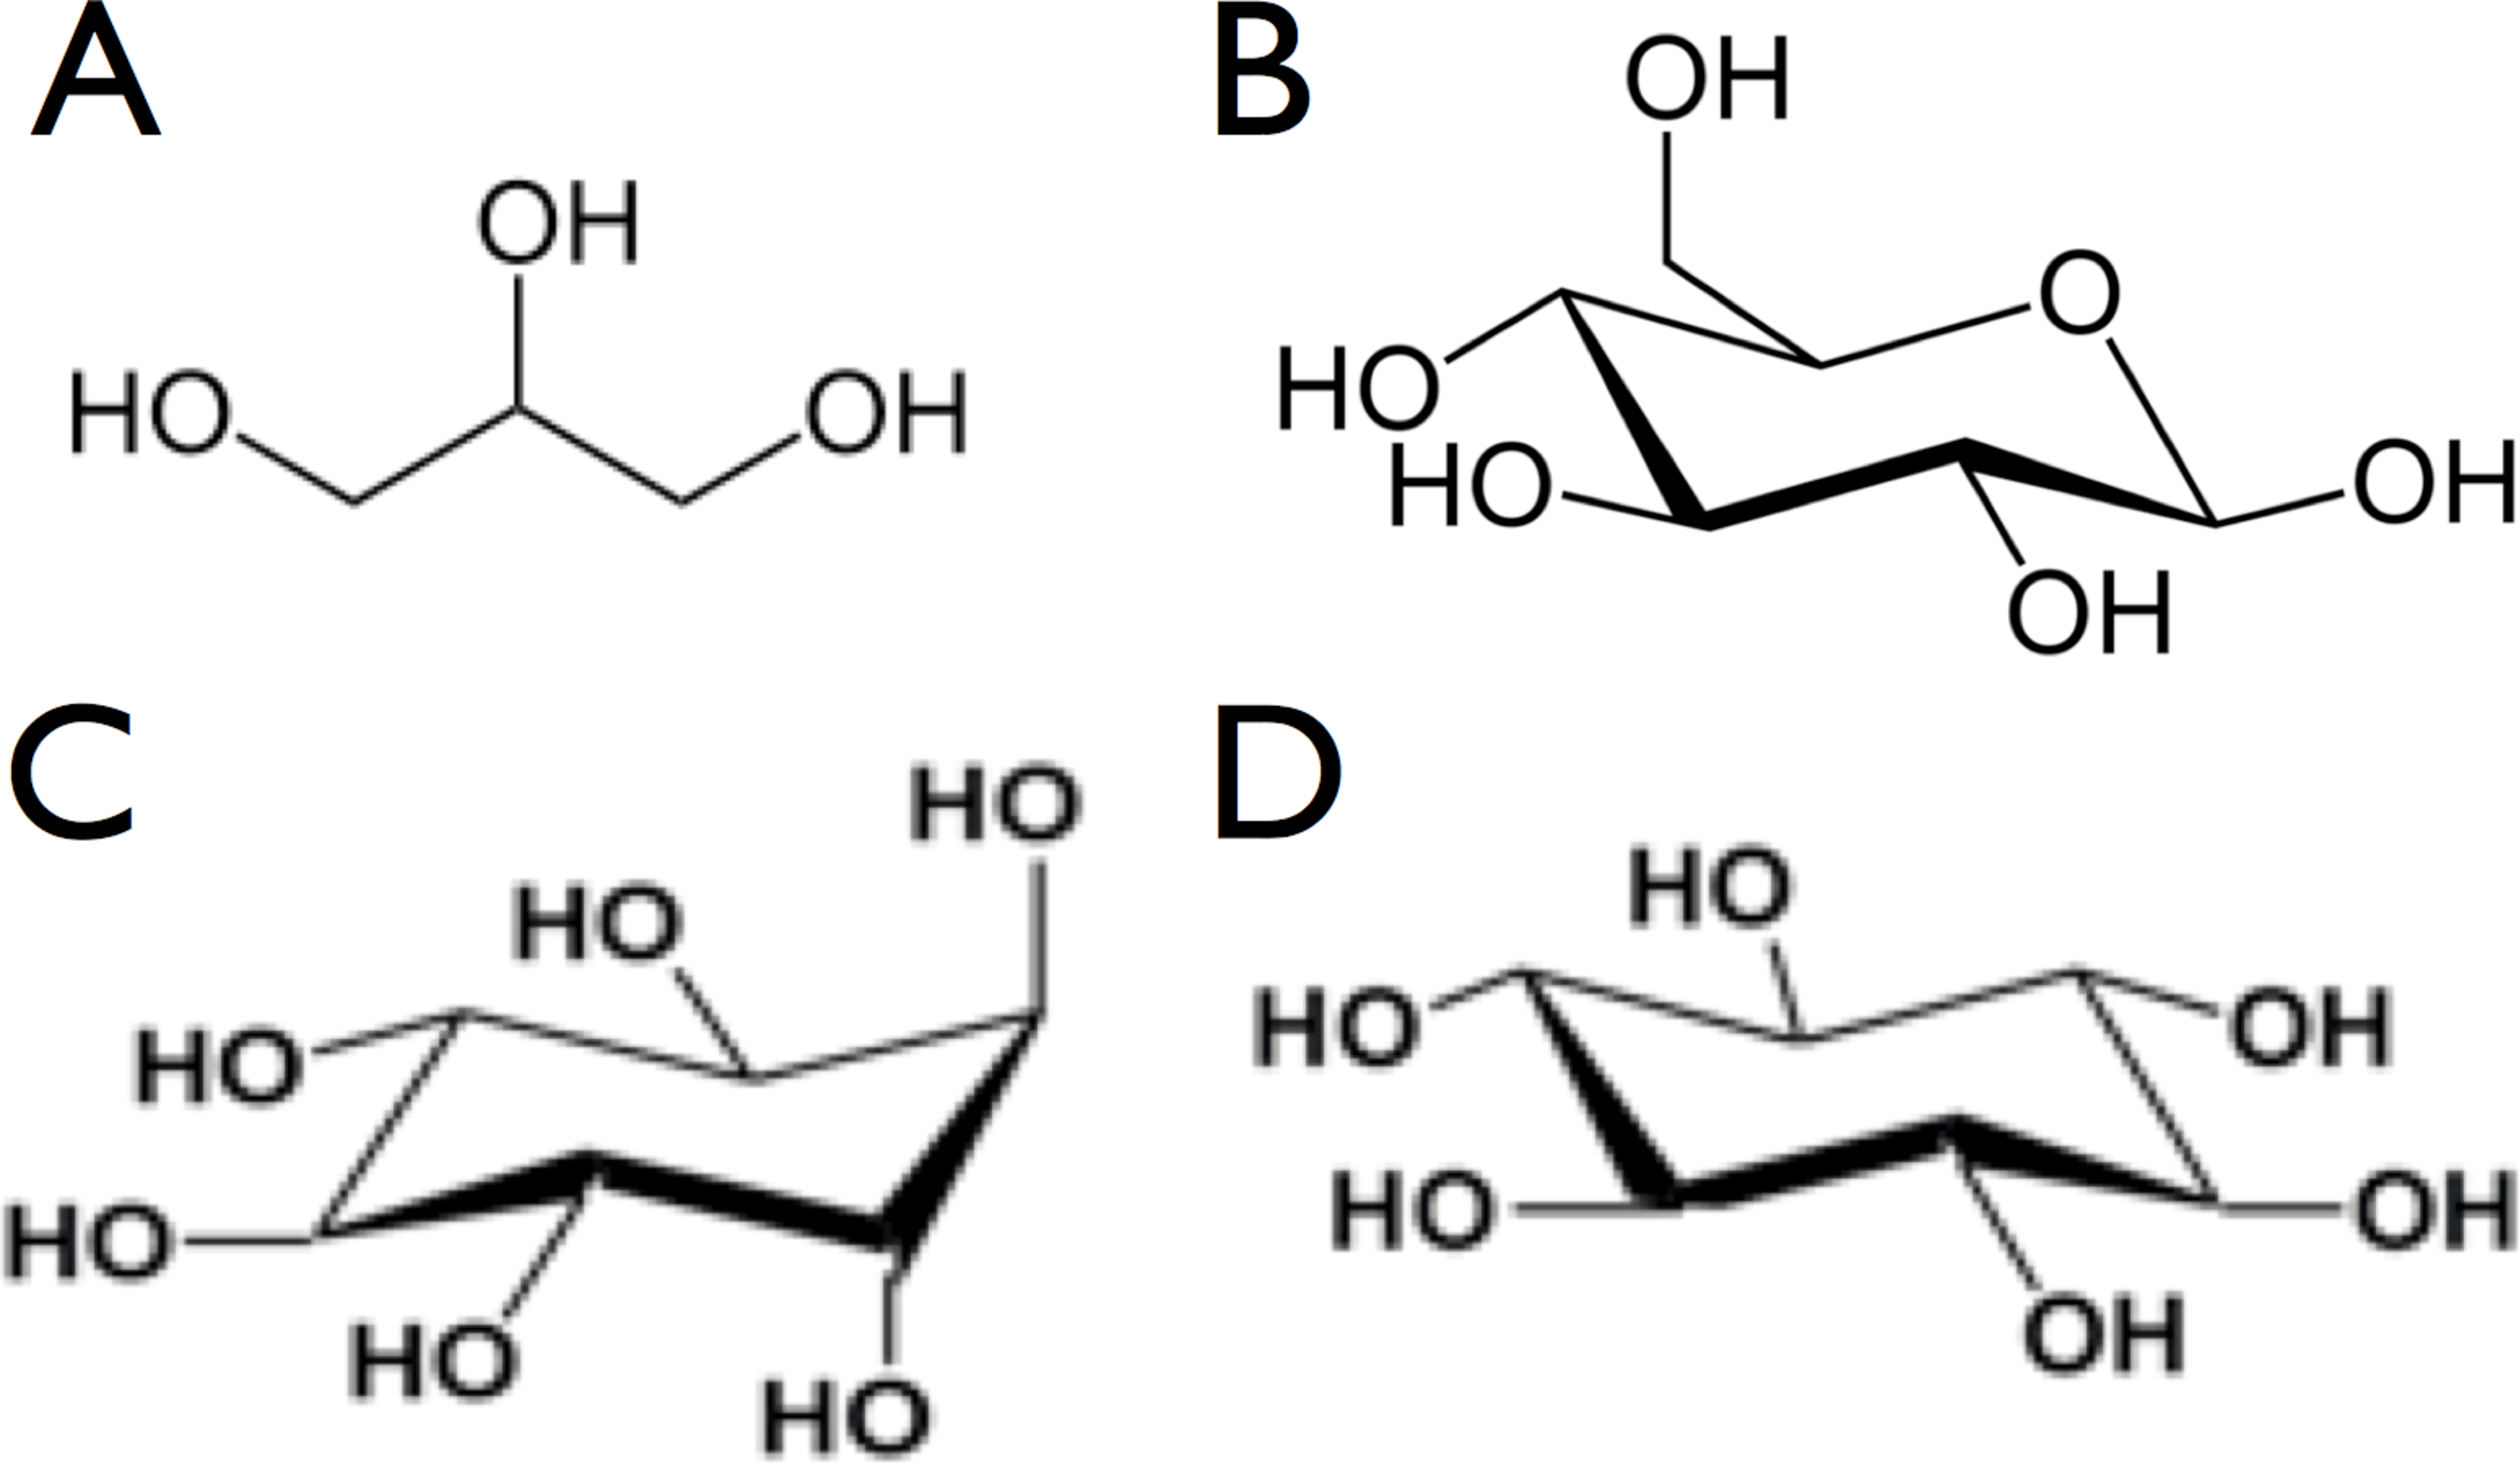
\includegraphics[width=2.5in]{figures/results3/ligands.pdf}
  \caption[Ligands]{Molecular structures of (A) glycerol, (B) glucose, (C) chiro-inositol and (D) scyllo-inositol}
  \label{fig:ligands}
\end{figure}

\begin{figure}[htbp]
  \centering
  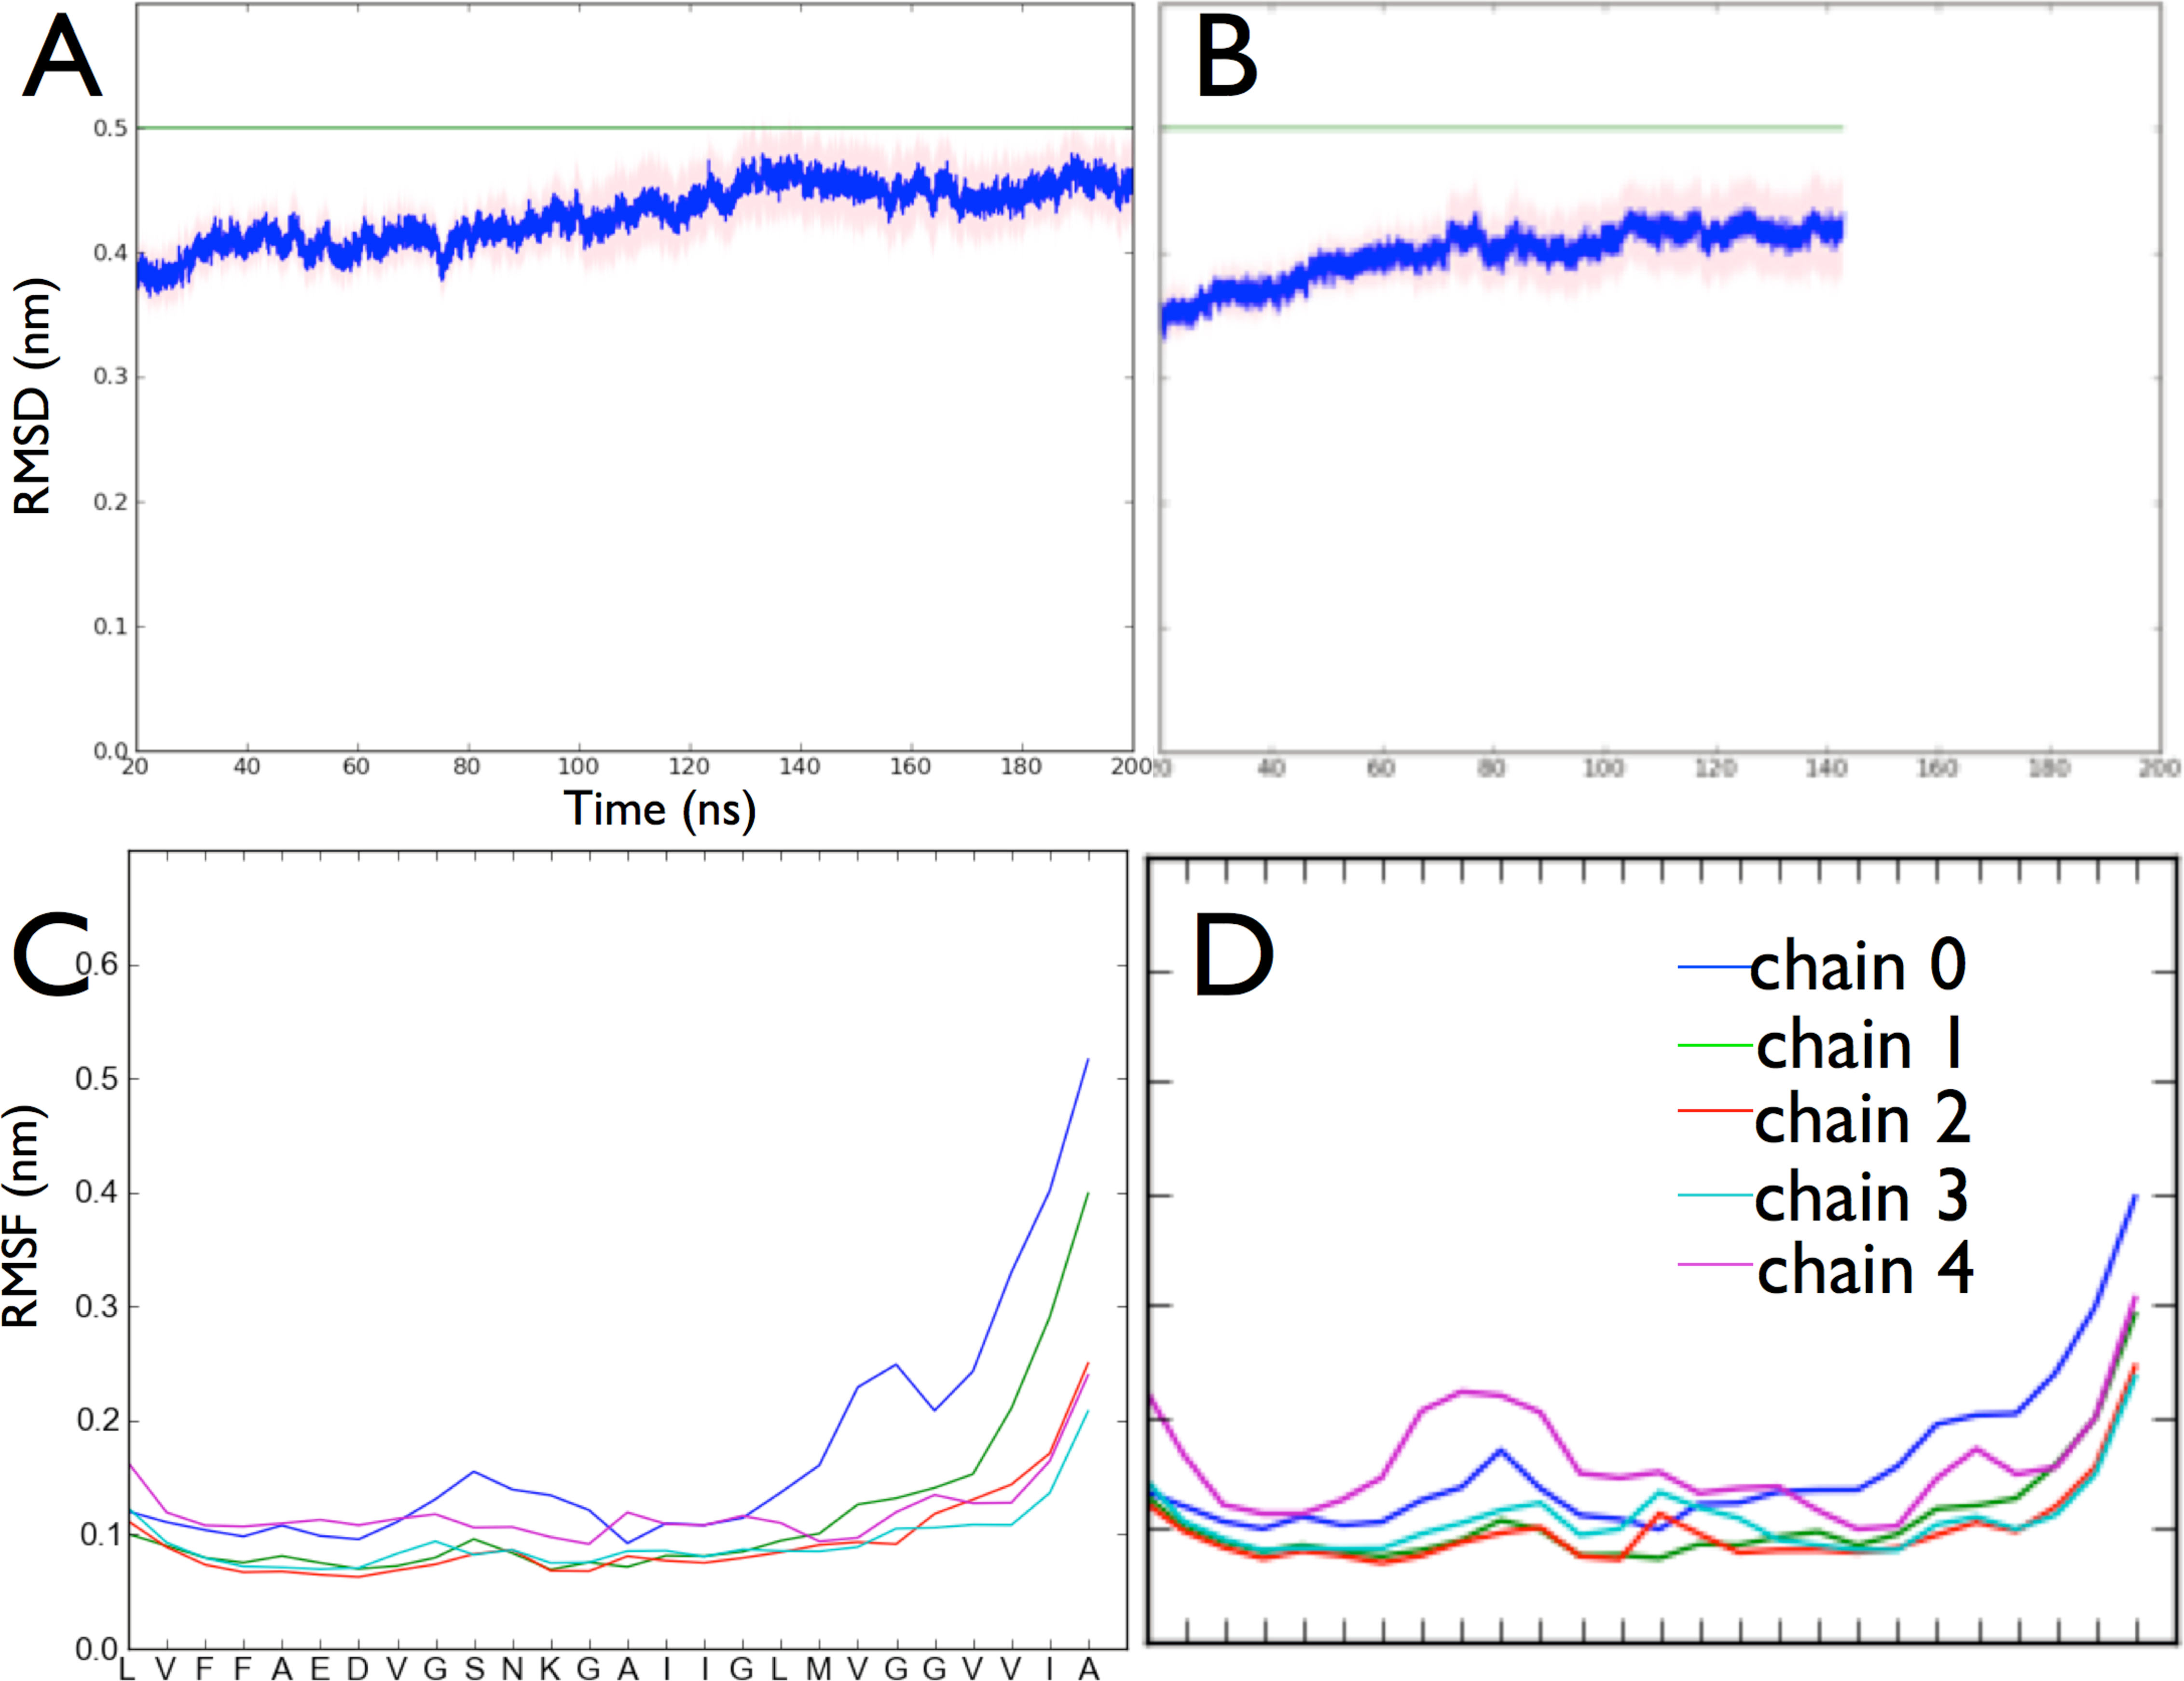
\includegraphics[width=5in]{figures/results3/protofibril_dynamics.pdf}
  \caption[RMSD and RMSF vs. time]{Fibril structure dynamics in pure water (A) and (C), and in the presence of scyllo-inositol (B) and (D).}
  \label{fig:protofibril_dynamics}
\end{figure}

\begin{figure}[htbp]
  \centering
  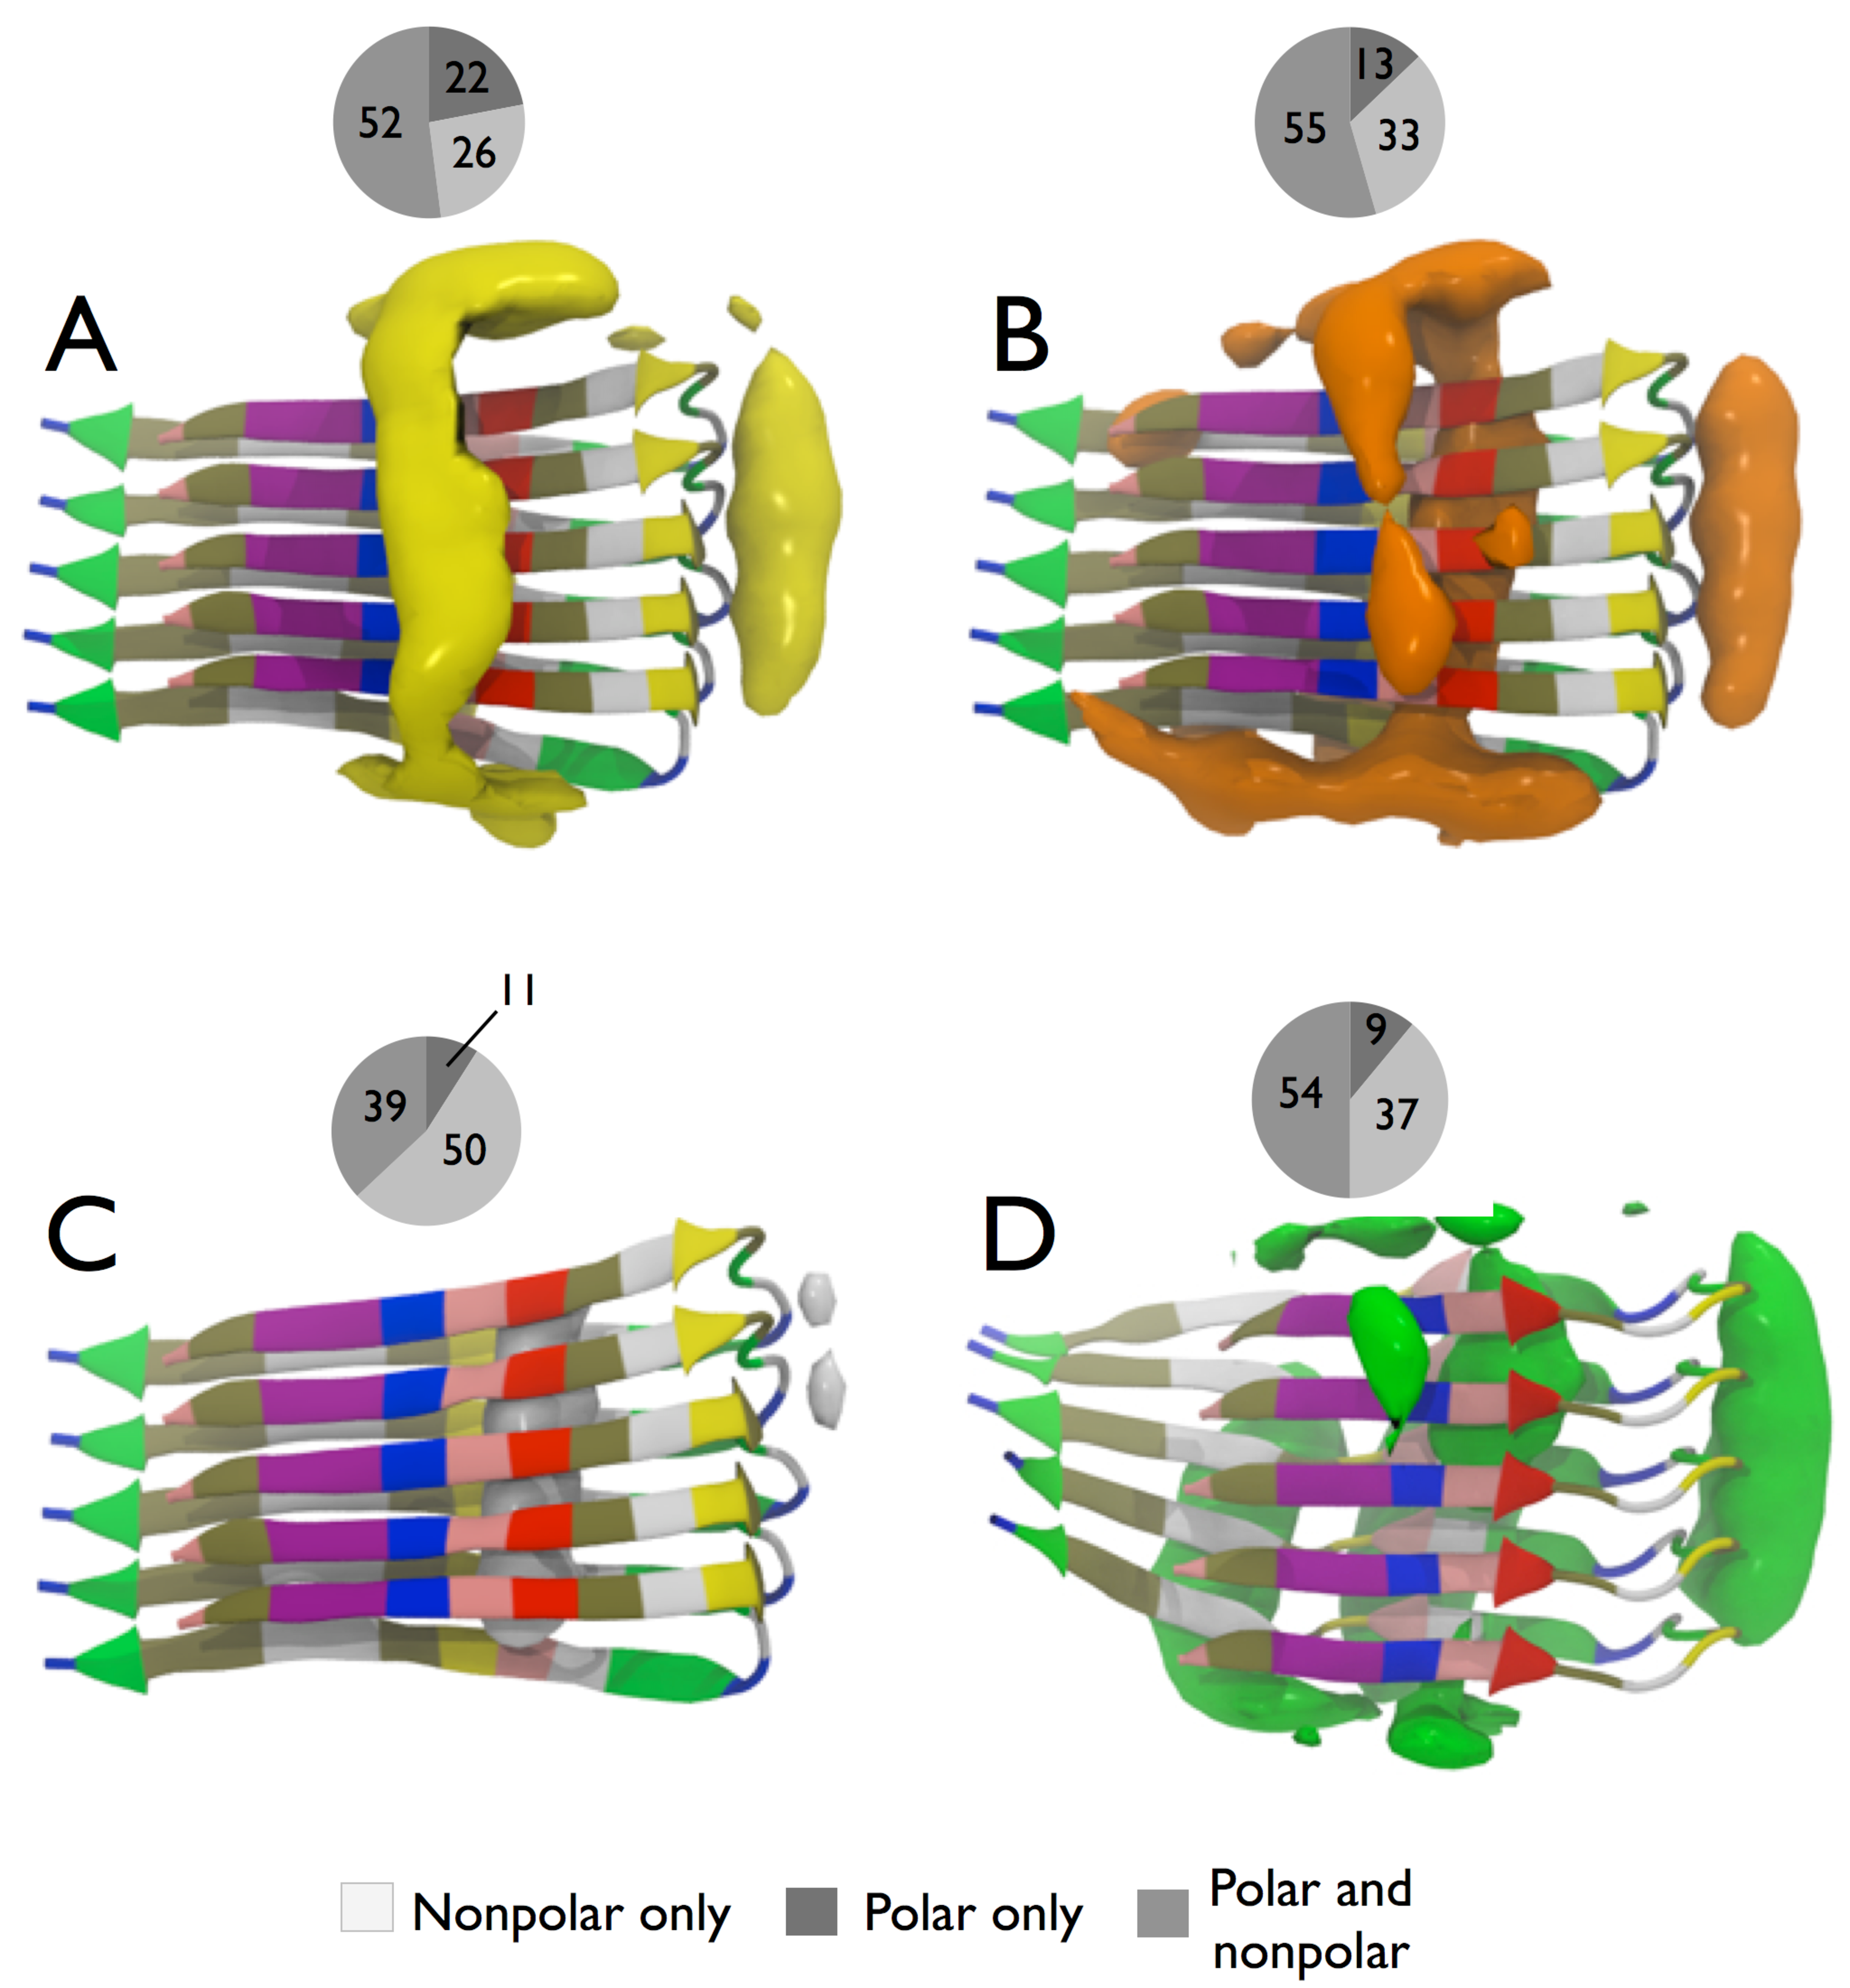
\includegraphics[width=6in]{figures/results3/binding_sdf_pie_chart.pdf}
  \caption[Abeta42 binding]{Comparisons of the spatial probability densities for (A) scyllo-inositol, (B) chiro-inositol (C) glycerol and (D) glucose.}
  \label{fig:spatial_binding}
\end{figure}

\begin{figure}[htbp]
  \centering
  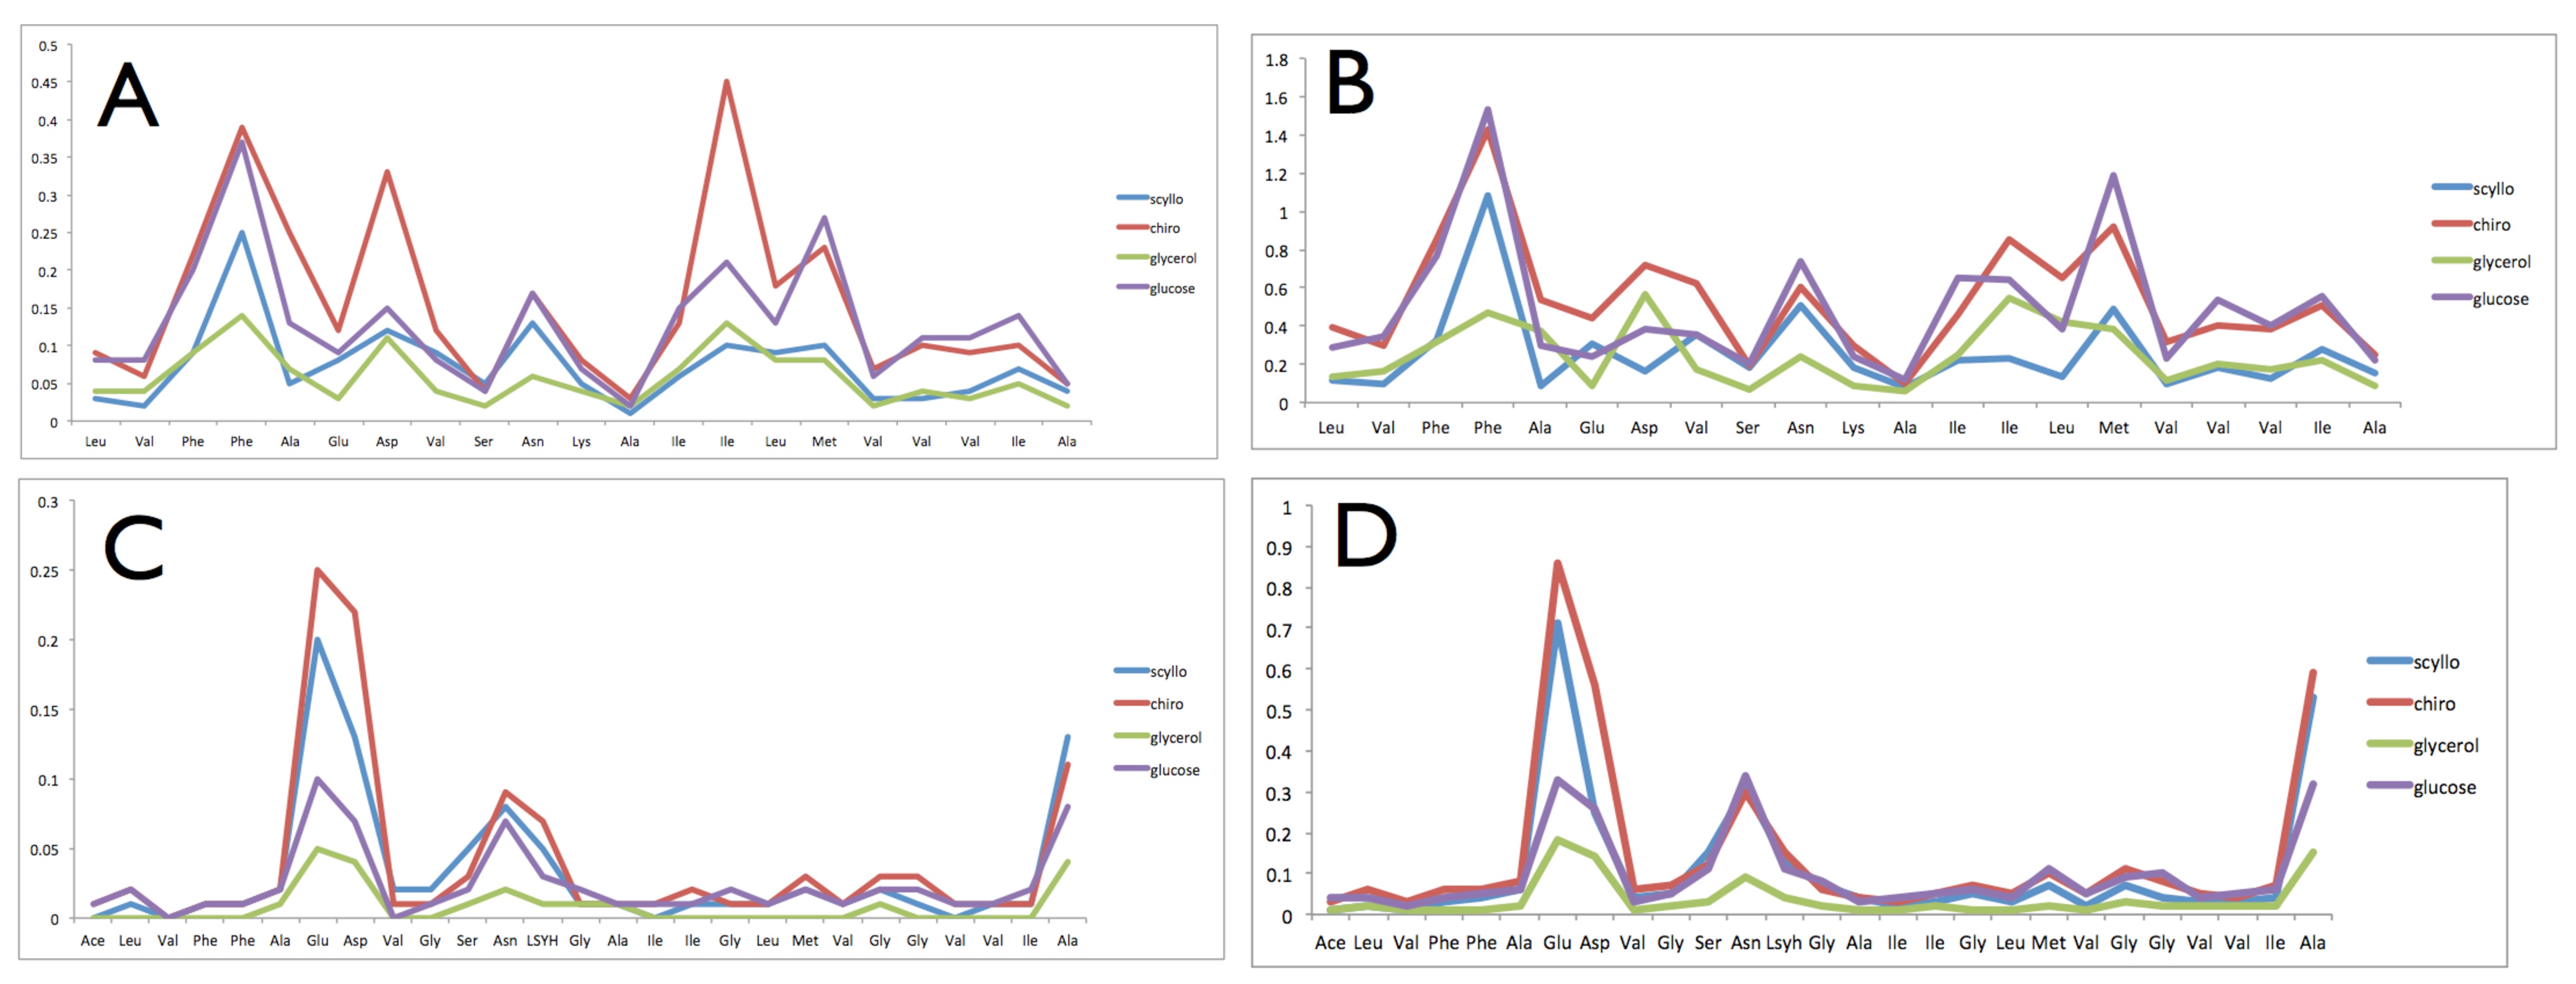
\includegraphics[width=6in]{figures/results3/binding_propensity_per_residue.pdf}
  \caption[Binding propensity]{Binding propensity per residue of scyllo-inositol, chiro-inositol, glycerol and glucose. Nonpolar binding propensities are depicted in (A) and (B), and hydrogen bonding propensities in (C) and (D).}
% Try to put nonpolar and hydrogen bonding for each ligand on separate panels. When put together it�s a little difficult to emphasize the differences
  \label{fig:binding_propensity}
\end{figure}

\begin{figure}[htbp]
  \centering
  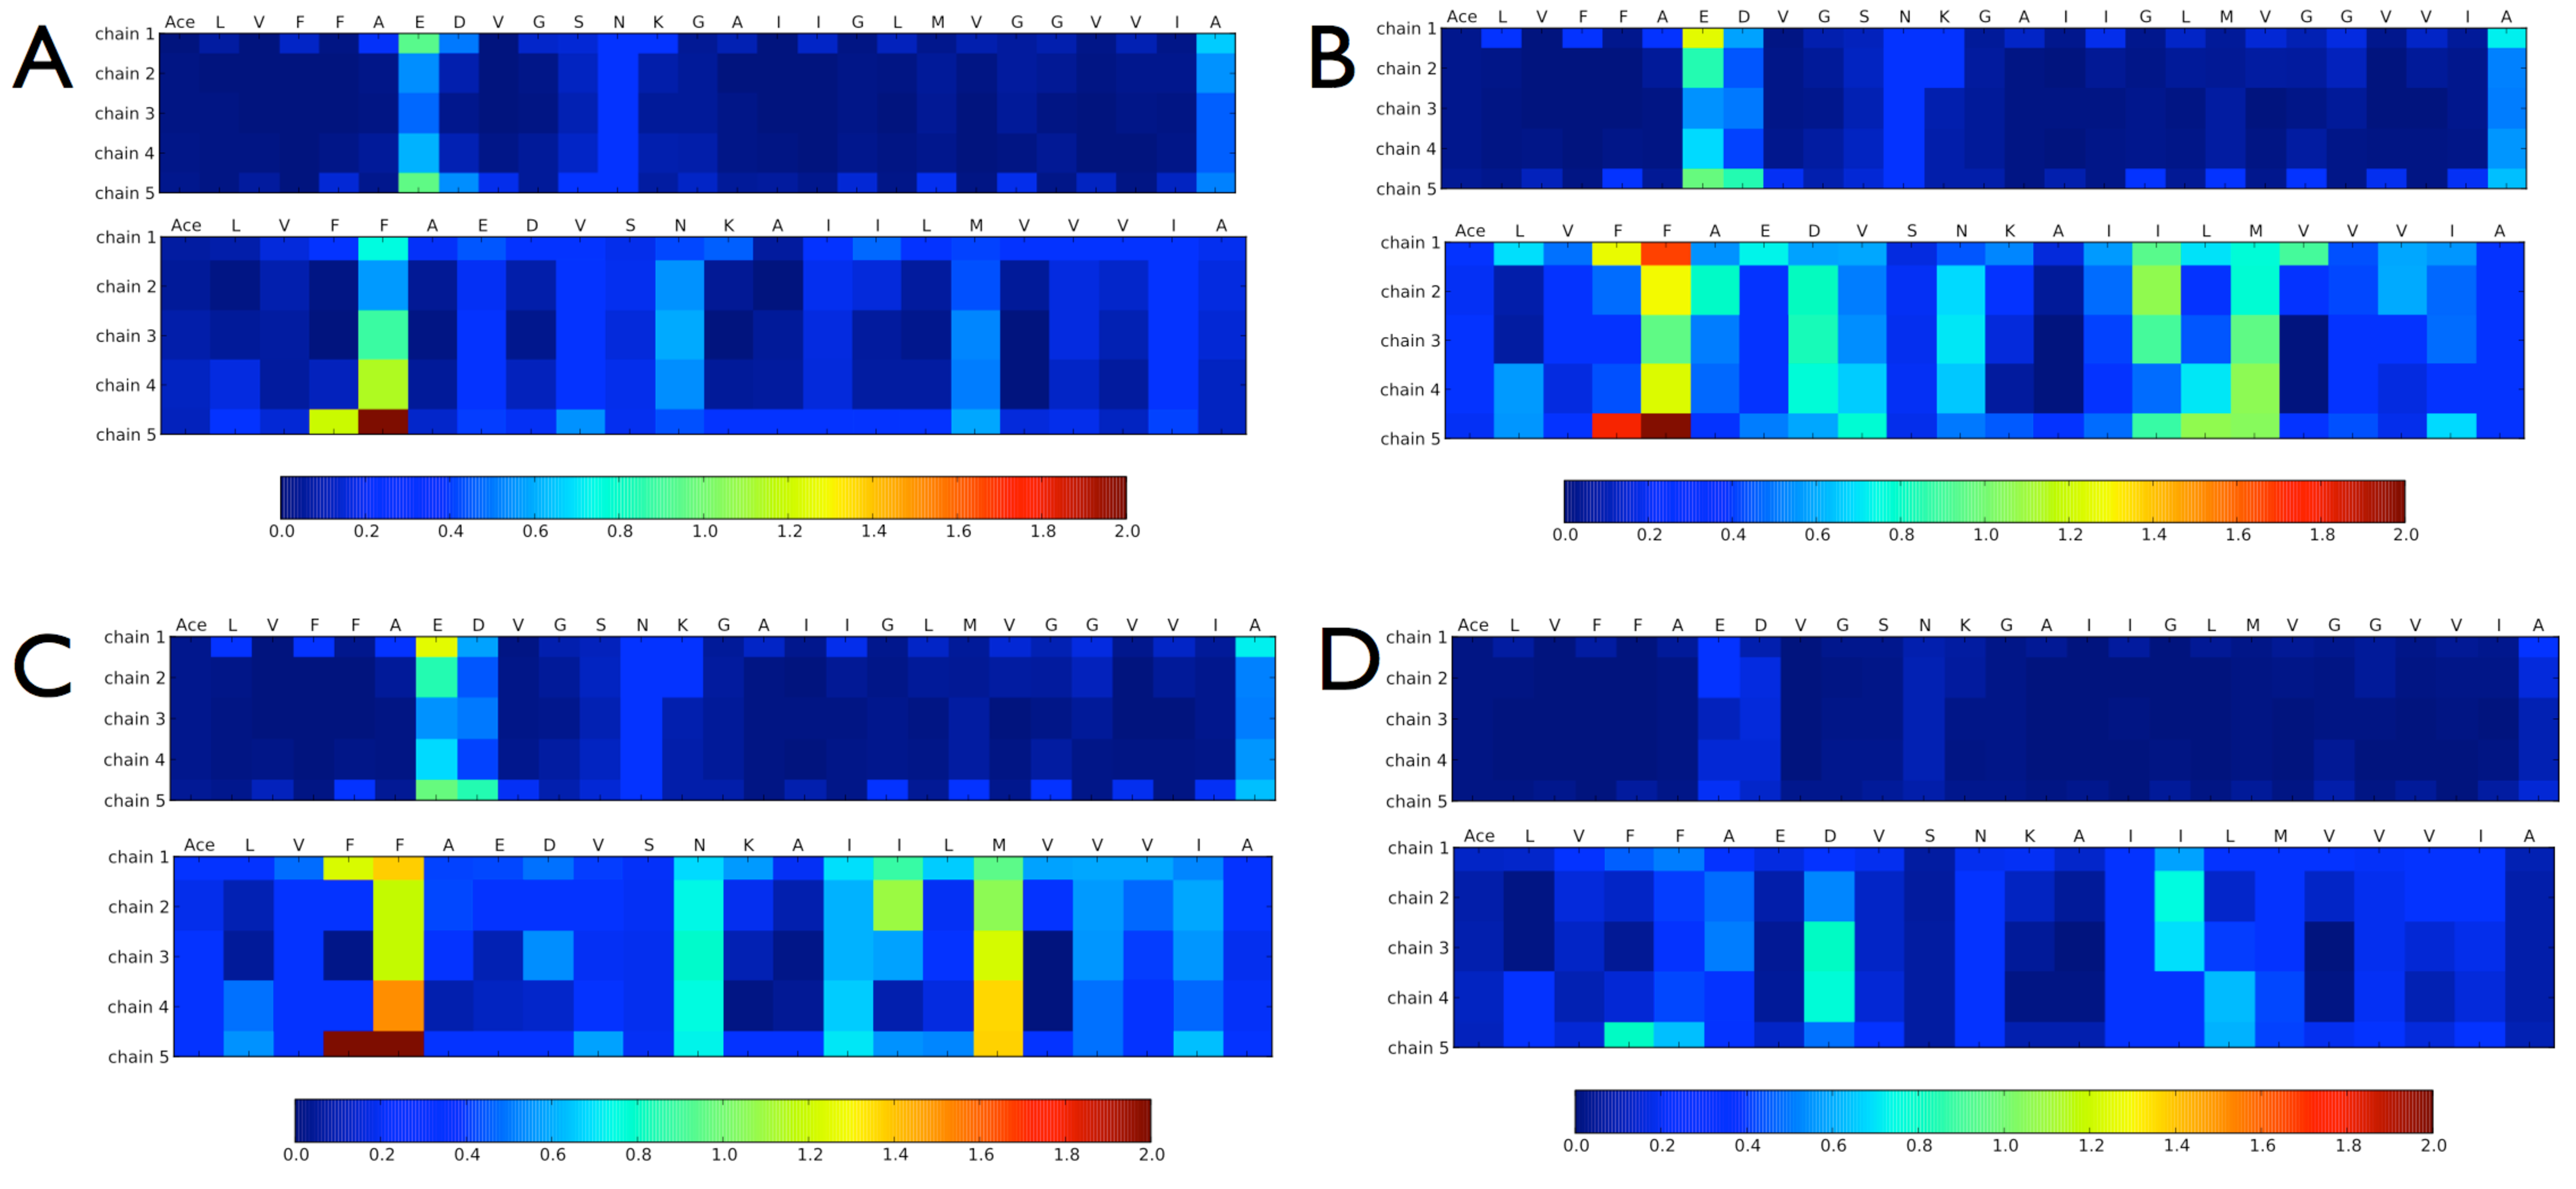
\includegraphics[width=6in]{figures/results3/binding_contact_map.pdf}
  \caption[Binding contact map]{Nonpolar and hydrogen bonding contact maps for the protofibril with (A) scyllo-inositol (B) chiro-inositol (C) glucose and (D) glycerol. The contact map for nonpolar and hydrogen bonding are shown on the top and bottom panels, respectively, for each solute.}
  \label{fig:binding_map}
\end{figure}

\begin{singlespace}
\addcontentsline{toc}{section}{Bibliography}
\bibliographystyle{elsart-num}
\bibliography{/Users/grace/github/thesis/document/results3/results3}
\end{singlespace}

